% la-05-leastsqu.tex

\documentclass[xcolor=dvipsnames]{beamer}
\usepackage{teachbeamer}

\title{Vectors}
\subtitle{{\CourseNumber}, BCIT}

\author{\CourseName}

\date{October 8, 2018}

\begin{document}

\begin{frame}
  \titlepage
\end{frame}

\begin{frame}
  \frametitle{Projection}
  The \alert{projection} $u_{H}$ of a vector $u$ onto a hyperplane $H$
  is the vector in the hyperplane that is ``most similar'' to $u$. The
  formal definition for $u_{H}$ requires that
  \begin{enumerate}
  \item $u$ is in $H$
  \item $(u-u_{H})$ is orthogonal to all basis vectors of $H$
  \end{enumerate}
\end{frame}

\begin{frame}
  \frametitle{Projection}
  \beispiel{Finding a Projection} Let $H$ be the line spanned by
  $\vec{v}=(-1,1)^{\intercal}$ in $\mathbb{R}^{2}$. What is the
  projection $\vec{w}$ of $\vec{u}=(3,-2)^{\intercal}$?
    \begin{figure}[h]
    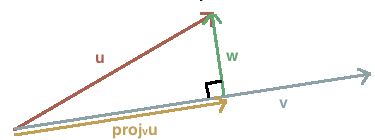
\includegraphics[scale=0.32]{./diagrams/project.png}
  \end{figure}
  Let $\vec{w}=(w_{1},w_{2})^{\intercal}$. Then (1) $\vec{u}-\vec{w}$
  is orthogonal to $\vec{v}$ and (2) $\vec{w}=\alpha\vec{v}$ for some
  $\alpha\in\mathbb{R}$.
  \begin{equation}
    \label{eq:vorahcat}
    \begin{array}{ccccc}
      w_{1}&-&w_{2}&=&5 \\
      w_{1}&+&w_{2}&=&0 \\
    \end{array}
  \end{equation}
Cramer's rule tells us that $\vec{w}=(2.5,-2.5)^{\intercal}$. 
\end{frame}

\begin{frame}
  \frametitle{Projection}
  Let $u=(u_{1},{\ldots},u_{n})^{\intercal}$ be a vector and $H$ be a
  $k$-dimensional hyperplane in the vector space $\mathbb{R}^{n}$. Let
  $x_{1},{\ldots},x_{k}$ be a basis for $H$. Then it is true for all
  vectors $v$ in the hyperplane that
  \begin{equation}
    \label{eq:ahdoogoh}
    \Vert{}u-v\Vert\geq\Vert{}u-u_{H}\Vert
  \end{equation}
  Proof: use the theorem of Pythagoras for
  \begin{equation}
    \label{eq:yoochaev}
    \Vert{}u-v\Vert^{2}=\Vert{}u-u_{H}\Vert^{2}+\Vert{}u_{H}-v\Vert^{2}\geq\Vert{}u-u_{H}\Vert^{2}
  \end{equation}
The claim follows. It illustrates what I mean when I say that $u_{H}$
is the vector in $H$ that is most similar to $u$. 
\end{frame}

\begin{frame}
  \frametitle{Projection}
  \beispiel{Finding Another Projection} What is the projection of
  $\vec{u}=(5,2,10)^{\intercal}$ onto the plane $T$ characterized by
  $2x+y+3z=0$?

  \medskip

  First we find two linearly independent vectors in $H$ to form a
  basis of $H$, for example $\vec{v_{1}}=(1,1,-1)^{\intercal}$ and
  $\vec{v_{2}}=(0,-3,1)^{\intercal}$. The conditions
  \begin{enumerate}
  \item $u_{H}\in{}T$
  \item $(u-u_{H})\perp{}v_{1}$
  \item $(u-u_{H})\perp{}v_{2}$
  \end{enumerate}
  give us the system of linear equations
  \begin{equation}
    \label{eq:faishiso}
    \left[
      \begin{array}{ccc}
        2 & 1 & 3 \\
        -1 & 1 & 1 \\
        0 & 3 & -1
      \end{array}\right]\cdot\left[
      \begin{array}{c}
        \hat{x} \\
        \hat{y} \\
        \hat{z}
      \end{array}\right]=\left[
      \begin{array}{c}
        0 \\
        3 \\
        -4
      \end{array}\right]
  \end{equation}
for which the solution is $u_{H}=(\hat{x},\hat{y},\hat{z})^{\intercal}=(-1,-1,1)^{\intercal}$.
\end{frame}

\begin{frame}
  \frametitle{Least Squares Method}
  Let there be two linearly independent vectors $u$ and $v$ in
  $\mathbb{R}^{n}$. Then the formula for the projection $u_{v}$ of $u$ onto
  the line spanned by $v$ is
  \begin{equation}
    \label{eq:weehohqu}
    u_{v}=\left(\frac{u\cdot{}v}{v\cdot{}v}\right)v
  \end{equation}
To verify the formula, note that $u_{v}=av$ for some real number $a$.
Therefore
\begin{equation}
  \label{eq:yahveego}
  (u-av)\perp{}v
\end{equation}
Isolate $a$ in the equation $(u-av)\cdot{}v=0$ to yield the formula.
\end{frame}

\begin{frame}
  \frametitle{Least Squares Method}
  Formula (\ref{eq:weehohqu}) only works when the hyperplane is a
  line. You can scale up the idea in terms of dimensions by the
  following theorem.
  \begin{block}{Formula for Projection Onto Plane with Orthogonal
      Basis}
    Let $\{u,v\}$ be an orthogonal basis for $H$. Then the projection
    of $w$ onto $H$ is the sum of $w_{u}$ and $w_{v}$, the projections
    of $w$ onto the lines spanned by $u$ and $v$, respectively.
  \end{block}
  Proof: check the following
  \begin{enumerate}
  \item $(w_{u}+w_{v})\in{}H$ (trivial)
  \item $(w-(w_{u}+w_{v}))\perp{}u$ (use the fact that $u\perp{}v$)
  \item $(w-(w_{u}+w_{v}))\perp{}v$ (same idea)
  \end{enumerate}
\end{frame}

\begin{frame}
  \frametitle{Least Squares Method}
  Consider the following table of measurements for the length of shoe
  prints and the height of the person wearing the shoes.

  \medskip
  
  \begin{tabular}{|c|c|}\hline
    Shoe Print (cm) & Height (cm) \\ \hline
    29.7 & 175.3 \\ \hline
    29.9 & 177.8 \\ \hline
    31.4 & 185.4 \\ \hline
    31.8 & 175.3 \\ \hline
    27.6 & 172.7 \\ \hline
  \end{tabular}

  \medskip
  
  In the statistics portion of this course, we will learn whether the
  paired data provide evidence of a linear relationship. In the linear
  algebra portion, we will learn how to find the line which is closest
  to the data points in the least squares sense.
\end{frame}

\begin{frame}
  \frametitle{Least Squares Method}
    \begin{figure}[h]
    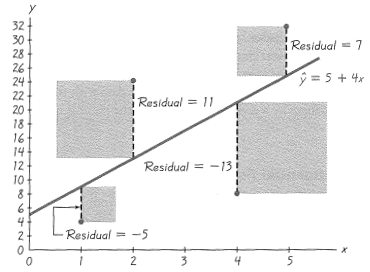
\includegraphics[scale=1]{./diagrams/lsqu4.png}
    \end{figure}
\end{frame}

% \begin{frame}
%   \frametitle{Least Squares Method}
%     \begin{figure}[h]
%     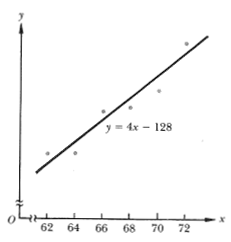
\includegraphics[scale=1]{./diagrams/lsqu1.png}
%     \end{figure}
% \end{frame}

% \begin{frame}
%   \frametitle{Least Squares Method}
%     \begin{figure}[h]
%     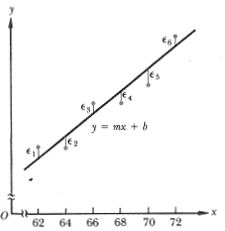
\includegraphics[scale=1]{./diagrams/lsqu3.png}
%     \end{figure}
% \end{frame}

\begin{frame}
  \frametitle{Least Squares Method}
  \begin{block}{Least Squares Method}
    If $L$ is a given line, the \alert{error} for each data point is
    the vertical distance from that point to the line. The
    \alert{squared error} is the sum of the squares of the errors. The
    line that best fits the data in the least squares sense is the
    line that minimizes the squared error.
  \end{block}

  \bigskip

  You can find the \alert{regression line} using calculus
  optimization. However, there is also an elegant method using linear
  algebra.
\end{frame}

\begin{frame}
  \frametitle{Least Squares Method}
  Let $L$ be a line with slope $m$ and $y$-intercept $b$. Let
  $(x_{1},y_{1}),(x_{2},y_{2}),{\ldots},(x_{n},y_{n})$ be a set of
  paired data. Then the following equations hold:
  \begin{equation}
    \label{eq:cheexame}
    \begin{array}{ccccccc}
      y_{1}&=&mx_{1}&+&b&+&\epsilon_{1} \\
      y_{2}&=&mx_{2}&+&b&+&\epsilon_{2} \\
      &&&{\vdots}&&& \\
      y_{n}&=&mx_{n}&+&b&+&\epsilon_{n} \\
    \end{array}
  \end{equation}
where the $\epsilon_{i}$ are the errors ($i=1,{\ldots},n$). This
system is equivalent to the following vector equation,
\begin{equation}
  \label{eq:aewieley}
  Y=AV+E
\end{equation}
where $Y,A,V,E$ are defined on the next slide.
\end{frame}

\begin{frame}
  \frametitle{Least Squares Method}
  \begin{equation}
    \label{eq:aikaewah}
    Y=\left[
      \begin{array}{cc}
        y_{1}  \\
        y_{2}  \\
        {\vdots} \\
        y_{n}  
      \end{array}\right],
    A=\left[
      \begin{array}{cc}
        x_{1} & 1 \\
        x_{2} & 1 \\
        {\vdots} & {\vdots} \\
        x_{n} & 1
      \end{array}\right],
    V=\left[
      \begin{array}{cc}
        m  \\
        b  
      \end{array}\right],
    E=\left[
      \begin{array}{cc}
        \epsilon_{1}  \\
        \epsilon_{2}  \\
        {\vdots} \\
        \epsilon_{n}  
      \end{array}\right]\notag
  \end{equation}
  $E$ is called the error vector. According to (\ref{eq:aewieley}), it
  is
  \begin{equation}
    \label{eq:keebiero}
    E=Y-AV
  \end{equation}
  We are trying to choose $m,b$ so that
  \begin{equation}
    \label{eq:phugeyai}
    \Vert{}E\Vert^{2}=\Vert{}Y-AV\Vert^{2}
  \end{equation}
is minimal.
\end{frame}

\begin{frame}
  \frametitle{Least Squares Method}
  Let
  \begin{equation}
    \label{eq:iapuveer}
    X=\left[
      \begin{array}{c}
        x_{1} \\
        {\vdots} \\
        x_{n}
      \end{array}\right]\mbox{ and }B=\left[
      \begin{array}{c}
        1 \\
        {\vdots} \\
        1
      \end{array}\right]
  \end{equation}
  Then $AV=mX+bB$. The set $S=\{AV|m,b\in\mathbb{R}\}$ is a plane in
  $n$-dimensional space. The ordered pair $(m,b)$ that minimizes the
  squared error corresponds to the projection $Y_{S}$ of $Y$ onto $S$.
\end{frame}

\begin{frame}
  \frametitle{Least Squares Method}
  Let $C$ be $B-B_{X}$, where $B_{X}$ is the projection of $B$ onto
  the line spanned by $X$. Then
  \begin{equation}
    \label{eq:aiwaozie}
    C=B-\left(\frac{B\cdot{}X}{X\cdot{}X}\right)X
  \end{equation}
  Note that $X\perp{}C$. $X$ and $C$ form an orthogonal basis for $S$.
  We have chosen $C$ by a process called \alert{successive orthogonal
    selection}. Consequently,
  \begin{equation}
    \label{eq:eijohkah}
    Y_{S}=Y_{X}+Y_{C}=\left(\frac{Y\cdot{}X}{X\cdot{}X}\right)X+\left(\frac{Y\cdot{}C}{C\cdot{}C}\right)C
  \end{equation}
\end{frame}

\begin{frame}
  \frametitle{Least Squares Method}
  Replace the rightmost $C$ by $B-\left(\frac{B\cdot{}X}{X\cdot{}X}\right)X$ for
  \begin{equation}
    \label{eq:maigeise}
    Y_{S}=\left(\frac{Y\cdot{}X}{X\cdot{}X}-\left(\frac{Y\cdot{}C}{C\cdot{}C}\right)\left(\frac{B\cdot{}X}{X\cdot{}X}\right)\right)X+\left(\frac{Y\cdot{}C}{C\cdot{}C}\right)B
  \end{equation}
  or alternatively
  \begin{equation}
    \label{eq:soguesee}
    m=\frac{Y\cdot{}X}{X\cdot{}X}-\left(\frac{Y\cdot{}C}{C\cdot{}C}\right)\left(\frac{B\cdot{}X}{X\cdot{}X}\right)
  \end{equation}
  \begin{equation}
    \label{eq:cuboonai}
    b=\frac{Y\cdot{}C}{C\cdot{}C}
  \end{equation}
  with
  \begin{equation}
    \label{eq:nesheeli}
    C=B-\left(\frac{B\cdot{}X}{X\cdot{}X}\right)X
  \end{equation}
\end{frame}

\begin{frame}
  \frametitle{Angles at Gray Cliff}
  \beispiel{Angles at Gray Cliff} This example is from \mbox{Oscar S.
    Adams's} \emph{Application of the Theory of Least Squares to the
    Adjustment of Triangulation} (1915), a ``working manual for the
  computer in the office.'' You measure the following angles.

  \medskip
  
  \begin{tabular}{|c|c|c|}\hline
    from & to & angle \\ \hline
    Boulder & Tower & $65^{\circ}6'29.3''$ \\ \hline
    Tower & Tyonek & $19^{\circ}46'26.9''$ \\ \hline
    Tyonek & Round Point & $8^{\circ}39'14.2''$ \\ \hline
    Round Point & Boulder & $266^{\circ}27'47.9''$ \\ \hline
    % Boulder & Round Point & $93^{\circ}32'9.6''$ \\ \hline
  \end{tabular}
\end{frame}

\begin{frame}
  \frametitle{Angles at Gray Cliff}
  Notice that the angles do not add up to $360^{\circ}$. We are
  missing $1.7''$. How should we adjust these numbers?

  \medskip

  Basic assumptions underlying least squares theory in surveying are
  \begin{enumerate}
  \item mistakes and systematic errors have been eliminated
  \item the number of observations being adjusted is large
  \item the frequency distribution of the errors is normal
  \end{enumerate}
\end{frame}

\begin{frame}
  \frametitle{Angles at Gray Cliff}
  Convert the angles to real numbers
  \begin{equation}
    \label{eq:maeshoga}
    \hat{a}=65.108,\hat{b}=19.774,\hat{c}=8.6539,\hat{d}=266.46
  \end{equation}
  The sum is $359.999527778$. Here is a system of equations with
  measurement errors, exploiting the fact that $d$ is supposed to be
  $360^{\circ}-(a+b+c)$
\begin{equation}
  \label{eq:puzeiboo}
  \begin{array}{ccc}
    a&=&65.108+\epsilon_{1} \\
    b&=&19.774+\epsilon_{2} \\
    c&=&8.6539+\epsilon_{3} \\
    360-(a+b+c)&=&266.46+\epsilon_{4}
  \end{array}
\end{equation}
\end{frame}

\begin{frame}
  \frametitle{Angles at Gray Cliff}
The system of equations is equivalent to the following matrix
equation.
\begin{equation}
  \label{eq:ijuniero}
  \left[
    \begin{array}{ccc}
      1 & 0 & 0 \\
      0 & 1 & 0 \\
      0 & 0 & 1 \\
      -1 & -1 & -1
    \end{array}\right]\left[
    \begin{array}{c}
      a \\
      b \\
      c
    \end{array}\right]=\left[
    \begin{array}{c}
      65.108 \\
      19.774 \\
      8.6539 \\
      -93.537
    \end{array}\right]+\left[
    \begin{array}{c}
      \epsilon_{1} \\
      \epsilon_{2} \\
      \epsilon_{3} \\
      \epsilon_{4}
    \end{array}\right]
\end{equation}
In symbols,
\begin{equation}
  \label{eq:eceesien}
  AV=Y+E
\end{equation}
Again, we want to minimize
\begin{equation}
  \label{eq:ahgaituc}
  \Vert{}Y-AV\Vert^{2}=\Vert{}E\Vert^{2}
\end{equation}
\end{frame}

\begin{frame}
  \frametitle{Angles at Gray Cliff}
  The minimization is achieved by projecting $Y$ onto the hyperplane $S$
  \begin{equation}
    \label{eq:shohyaec}
    a\left[
      \begin{array}{c}
        1 \\
        0 \\
        0 \\
        -1
      \end{array}\right]+b\left[
      \begin{array}{c}
        0 \\
        1 \\
        0 \\
        -1
      \end{array}\right]+c\left[
      \begin{array}{c}
        0 \\
        0 \\
        1 \\
        -1
      \end{array}\right]
  \end{equation}
  These three vectors $\alpha,\beta,\gamma$ form a basis of $S$, but
  the basis vectors are not orthogonal to each other. We will search
  for a different basis of $S$ that is orthonormal by successive
  orthogonal selection.
\end{frame}

\begin{frame}
  \frametitle{Angles at Gray Cliff}
  Start with a non-zero vector $b_{1}$ in $S$, for example
  $b_{1}=\alpha=(1,0,0,-1)^{\intercal}$. This is our first basis
  vector. The second basis vector $b_{2}=x\alpha+y\beta+z\gamma$ must
  fulfill
  \begin{enumerate}
  \item $b_{2}\cdot{}b_{1}=0$ (which is equivalent to
    $b_{2}\perp{}b_{1}$)
  \item $b_{2}\in{}S$
  \end{enumerate}
For example, $b_{2}=(1,-1,-1,1)^{\intercal}$ qualifies. Follow the
same procedure for $b_{3}=(0,1,-1,0)^{\intercal}$.
\end{frame}

\begin{frame}
  \frametitle{Angles at Gray Cliff}
  Let $Y_{i}$ be the projection of $Y$ onto the line spanned by
  $b_{i}$, for example. 
  \begin{equation}
    \label{eq:zeoyeobe}
    Y_{1}=\left(\frac{Y\cdot{}b_{1}}{b_{1}\cdot{}b_{1}}\right)b_{1}=\left[
      \begin{array}{c}
        79.32242 \\
        0 \\
        0 \\
        -79.32242
      \end{array}\right]
  \end{equation}
  Then the projection $Y_{S}$ equals $Y_{1}+Y_{2}+Y_{3}=$
  \begin{equation}
    \label{eq:yeeyaesh}
    \left[
      \begin{array}{c}
        79.32242 \\
        0 \\
        0 \\
        -79.32242
      \end{array}\right]+\left[
      \begin{array}{c}
        -14.214 \\
        14.214 \\
        14.214 \\
        -14.214
      \end{array}\right]+\left[
      \begin{array}{c}
        0 \\
        5.56010 \\
        -5.56010 \\
        0
      \end{array}\right]=\left[
      \begin{array}{c}
        65.1083 \\
        19.7743 \\
        8.6541 \\
        -93.5366
      \end{array}\right]\notag
  \end{equation}
  The least squares adjusted angles are
  $65^{\circ}6'29.7'',19^{\circ}46'27.3'',8^{\circ}39'14.6''$ compared
  to the original
  $65^{\circ}6'29.3'',19^{\circ}46'26.9'',8^{\circ}39'14.2''$.
\end{frame}

\begin{frame}
  \frametitle{End of Lesson}
Next Lesson: Eigenvalues and Eigenvectors
\end{frame}

\end{document}

